% Appendix Template

\newcommand{\major}{4}
\newcommand{\minor}{1}

\newcommand{\undPrefix}{\major_\minor}
\newcommand{\dotPrefix}{\major.\minor}
\newcommand{\scoPrefix}{\major-\minor}
\newcommand{\filePrefix}{\undPrefix}

% \chapter{Results of experiment 1.1} % Main appendix title
\chapter{Results of experiment \dotPrefix} % Main appendix title

% \label{Appendix1-1} % Change X to a consecutive letter; for referencing this appendix elsewhere, use \ref{AppendixX}

\label{Appendix\scoPrefix} % Change X to a consecutive letter; for referencing this appendix elsewhere, use \ref{AppendixX}

These experiments are discussed \hyperref[disc:h4]{here}
\begin{figure}[ht]
  \centering
  \begin{subfigure}[t]{0.5\linewidth}
    % \centering\captionsetup{width=.8\linewidth}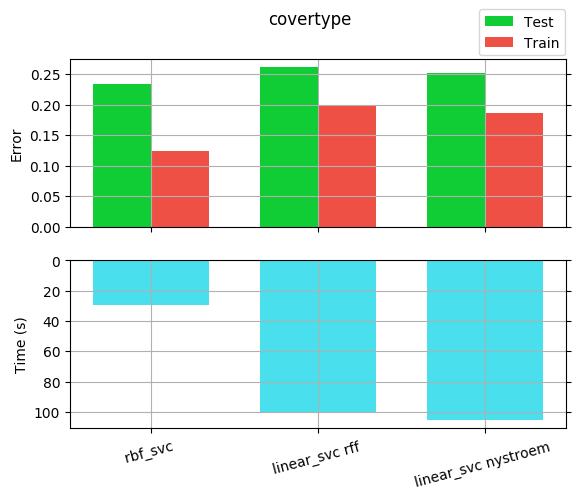
\includegraphics[width=\imgscale\linewidth]{Figures/1_1/covertype}
    \centering\captionsetup{width=.8\linewidth}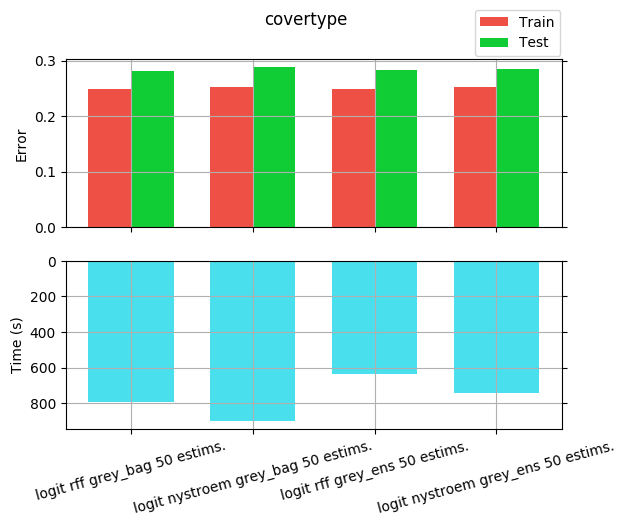
\includegraphics[width=\imgscale\linewidth]{Figures/\filePrefix/covertype}
    \caption{Exp. 4.1 with Covertype. Random Samplers increase the error on Decision Tree.}
    \label{fig:\undPrefix_covertype}
  \end{subfigure}%
  \begin{subfigure}[t]{0.5\linewidth}
    \centering\captionsetup{width=.8\linewidth}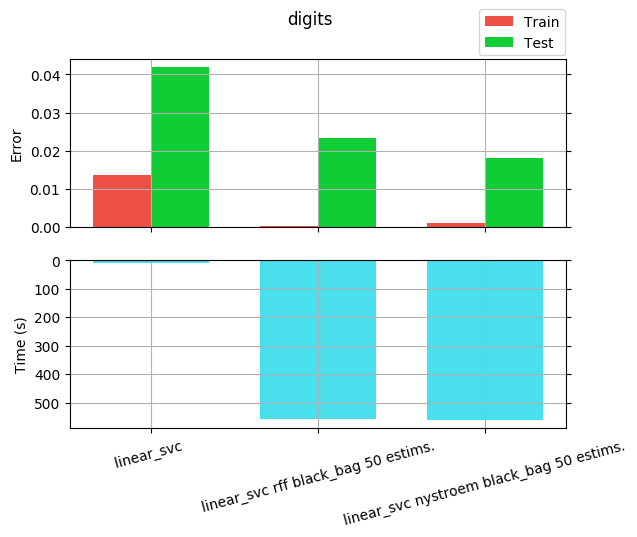
\includegraphics[width=\imgscale\linewidth]{Figures/\filePrefix/digits}
    \caption{Exp. 4.1 with Digits. Random Samplers increase the error on Decision Tree.}
    % \label{fig:1_1_digits}
    \label{fig:\undPrefix_digits}
  \end{subfigure}
\end{figure}


\begin{figure}[ht]
  \centering
  \begin{subfigure}[t]{0.5\linewidth}
    \centering\captionsetup{width=.8\linewidth}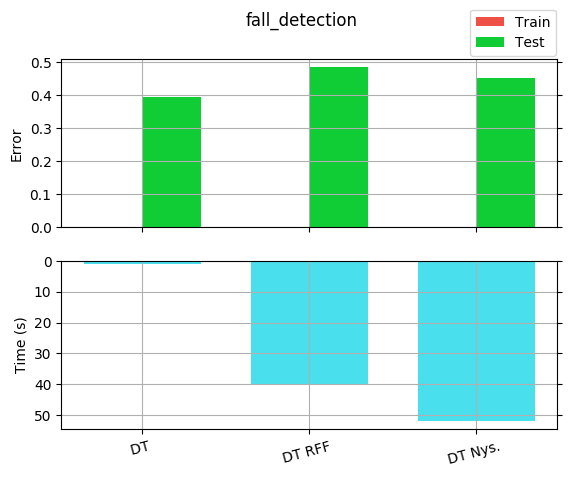
\includegraphics[width=\imgscale\linewidth]{Figures/\filePrefix/fall_detection}
    \caption{Exp. 4.1 with Fall Detection. Random Samplers increase the error on Decision Tree.}
    \label{fig:\undPrefix_fall_detection}
  \end{subfigure}%
  \begin{subfigure}[t]{0.5\linewidth}
    \centering\captionsetup{width=.8\linewidth}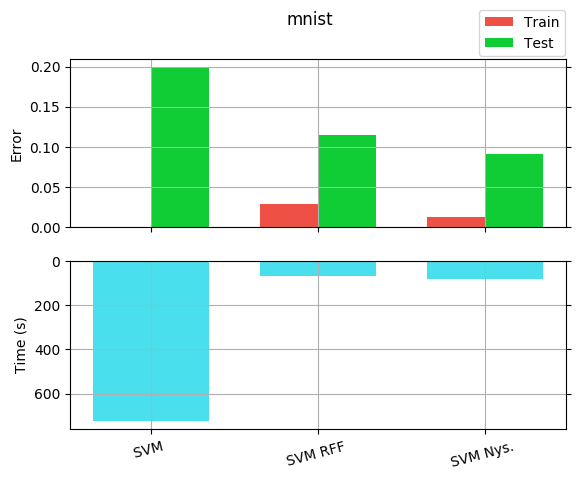
\includegraphics[width=\imgscale\linewidth]{Figures/\filePrefix/mnist}
    \caption{Exp. 4.1 with MNIST. Random Samplers increase the error on Decision Tree.}
    \label{fig:\undPrefix_mnist}
  \end{subfigure}
\end{figure}


\begin{figure}[ht]
  \centering
  \begin{subfigure}[t]{0.5\linewidth}
    \centering\captionsetup{width=.8\linewidth}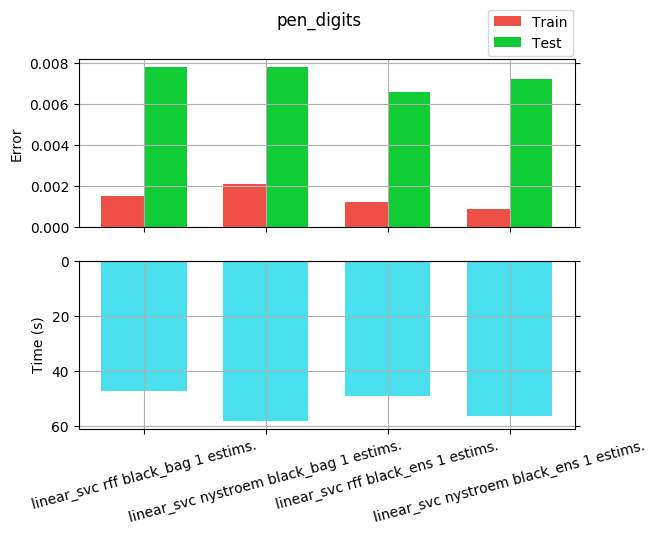
\includegraphics[width=\imgscale\linewidth]{Figures/\filePrefix/pen_digits}
    \caption{Exp. 4.1 with Pen Digits. Random Samplers increase the error on Decision Tree.}
    \label{fig:\undPrefix_pen_digits}
  \end{subfigure}%
  \begin{subfigure}[t]{0.5\linewidth}
    \centering\captionsetup{width=.8\linewidth}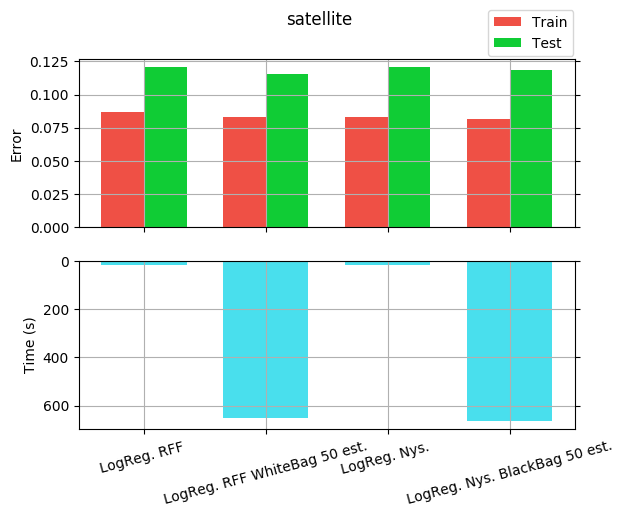
\includegraphics[width=\imgscale\linewidth]{Figures/\filePrefix/satellite}
    \caption{Exp. 4.1 with Satellite. Random Samplers make no difference on Decision Tree.}
    \label{fig:\undPrefix_satellite}
  \end{subfigure}
\end{figure}

\begin{figure}[ht]
  \centering
  \begin{subfigure}[t]{0.5\linewidth}
    \centering\captionsetup{width=.8\linewidth}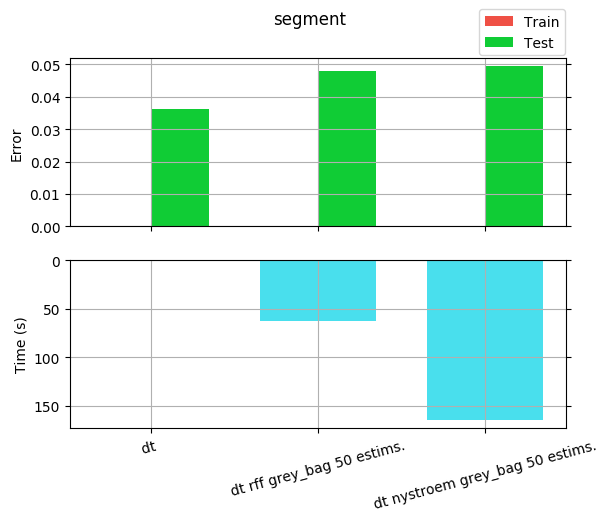
\includegraphics[width=\imgscale\linewidth]{Figures/\filePrefix/segment}
    \caption{Exp. 4.1 with Segment. Random Samplers increase the error on Decision Tree.}
    \label{fig:\undPrefix_segment}
  \end{subfigure}%
  \begin{subfigure}[t]{0.5\linewidth}
    \centering\captionsetup{width=.8\linewidth}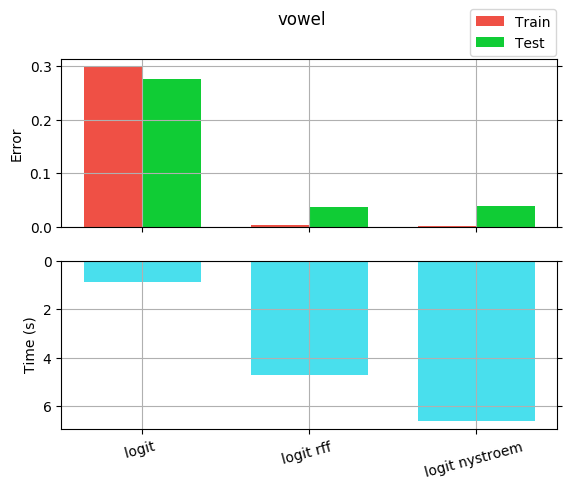
\includegraphics[width=\imgscale\linewidth]{Figures/\filePrefix/vowel}
    \caption{Exp. 4.1 with Vowel. Random Samplers increase the error on Decision Tree.}
    \label{fig:\undPrefix_vowel}
  \end{subfigure}
\end{figure}


\begin{figure}[ht]
  \centering
  \begin{subfigure}[t]{0.5\linewidth}
    \centering\captionsetup{width=.8\linewidth}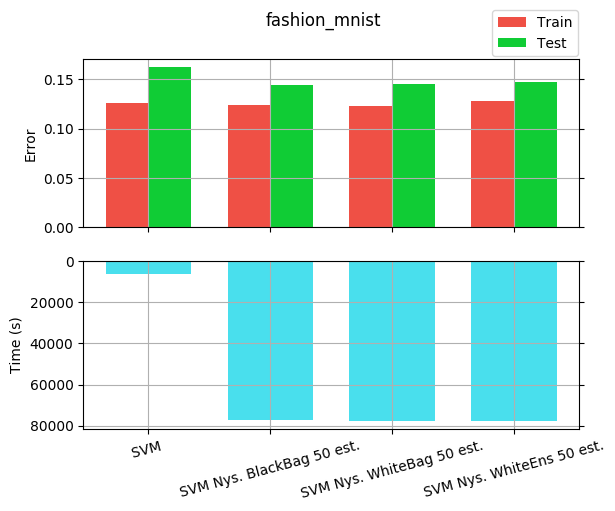
\includegraphics[width=\imgscale\linewidth]{Figures/\filePrefix/fashion_mnist}
    \caption{Exp. 4.1 with Fashion MNIST. Random Samplers increase the error on Decision Tree.}
    \label{fig:\undPrefix_segment}
  \end{subfigure}%
\end{figure}


\let\major\undefined
\let\minor\undefined

\let\undPrefix\undefined
\let\dotPrefix\undefined
\let\scoPrefix\undefined

\let\filePrefix\undefined
